\documentclass[10pt]{article}
\usepackage[T1]{fontenc}
\usepackage{lmodern,amsmath,amssymb,amsthm,booktabs,microtype}
\usepackage[margin=0.81in]{geometry}
\usepackage[colorlinks=true,urlcolor=blue,linkcolor=blue]{hyperref}
\usepackage{tikz}
\usetikzlibrary{arrows.meta,positioning}
\newtheorem{theorem}{Theorem}
\newtheorem{lemma}{Lemma}
\newtheorem{corollary}{Corollary}
\DeclareMathOperator{\ord}{ord}
\DeclareMathOperator{\Res}{Res}
\DeclareMathOperator{\Norm}{Norm}
\newcommand{\cat}{\mathbin{\Vert}}
\title{Spectral Compression of Decimal Mountain Concatenations:\\
Four Infinite Multiplicative-Order Families Beyond the Smooth Case}
\author{Qichao Wang}
\date{October 18, 2026 \quad \textit{computer-assisted partial result}}
\begin{document}\maketitle
\begin{abstract}
For \(M(k)=1\cat2\cat\cdots\cat k\cat(k-1)\cat\cdots\cat1\),
we prove that every prime \(p\) with
\(\ord_p(10)=7\cdot2^a5^c\) or
\(\ord_p(10)=11\cdot3^b2^a5^c\),
\(a,c\ge0,\ 0\le b\le2\),
divides at least one \(M(k)\).
The argument first compresses the stable affine drift for a
\emph{fixed} coprime-order component \(v\) to at most
\(\ell=\operatorname{lcm}(v,\ord_v(10))\) cyclotomic cosets,
uniformly over arbitrarily large powers of \(2,5\).
Both drift coordinates become polynomials of degree at most two
in \(m=r/\gcd(r,\ell)\) over a fixed-degree cyclotomic field.
Exact quadratic (\(v=7\)) and degenerate linear (\(v=11\))
resultants, followed by factorization-free cyclotomic sieves,
exclude simultaneous zero drift in these families.
A nine-torsion lifting lemma folds the new cases \(v=33,99\)
into the same 22-phase algebra as \(v=11\), reusing its norms.
This does not resolve the unrestricted OEIS A077187 conjecture.
\end{abstract}

\section{Affine drift and the period reduction}
For a prime \(p\nmid10\), set \(r=\ord_p(10)=uv\) with
\(u=2^a5^c\), \((v,10)=1\).
Write \(C_k=1\cat\cdots\cat k\),
\(Y_k=10^{-D(k)}(k\cat\cdots\cat1)\pmod p\),
where \(D(k)\) is the total digit count.
For a complete \(d\)-digit layer, put
\[
L=10^{d-1},\quad q=10^d,\quad n=9L,\quad A=q^n,
\quad S=\sum_{i<n}q^i,\quad J=\sum_{i<n}iq^i.
\]
The exact layer map is
\[
(C,Y)\longmapsto\bigl(AC+(q-1)S-J,\
A^{-1}(Y+LS+J)\bigr).
\]
The established stable-period lemma gives, for
\[
T=\operatorname{lcm}(r,\ord_v(10)),\qquad \ord_1(10)=1,
\]
a translation from the full block of digit layers \(T+1,\ldots,2T\).
Let \((U,V)\) denote its displacement.
If \((U,V)\ne(0,0)\), the normalized residues of
\(M(10^{jT})\), \(M(10^{jT}+1)\) have affine slopes
\(10U+V\) and \(1000U+V\). For \(p\ge7\), \(p\ne11\),
these cannot both vanish, yielding a divisible mountain with
\(1\le j\le p\).

Set \(h=\ord_v(10)\),
\[
\ell=\operatorname{lcm}(v,h),\qquad
g=\gcd(r,\ell),\qquad m=r/g,\qquad T=m\ell.
\]
The key point is that \(\ell\) depends only on \(v\), not on \(a,c\).

\begin{lemma}[Short-period phase]
For every stable digit layer \(d\), the diagonal multiplier
\(A_d=10^{9d10^{d-1}}\) has period \(\ell\).
Furthermore \(\prod_{j=d}^{d+\ell-1}A_j=1\pmod p\).
Thus its cumulative phase \(P_d\), started at \(d=T+1\),
also has period \(\ell\).
\end{lemma}
\begin{proof}
For stable \(d\), \(u\mid9d10^{d-1}\).
Modulo \(v\), periodicity follows from
\(v\mid\ell\) and \(10^\ell\equiv1\pmod v\).
For the product, use
\[
9\sum_{j=d}^{d+\ell-1}j10^{j-1}
=(d+\ell-1)10^{d+\ell-1}-d10^{d-1}
-\sum_{j=d}^{d+\ell-2}10^j.
\]
The exponent is zero modulo \(u\) termwise and modulo \(v\)
because \(v\mid\ell\) and \(v\mid(10^\ell-1)/9\);
the latter follows from the lifting-the-exponent identity at \(3\)
and invertibility of \(9\) at the remaining prime divisors.
Therefore \(r\) divides the full exponent.
\end{proof}

\begin{figure}[h]
\centering
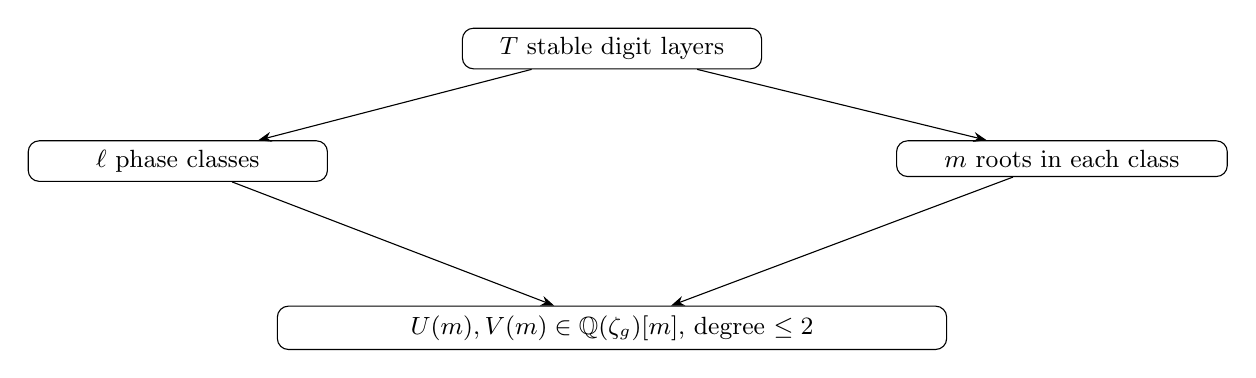
\begin{tikzpicture}[>=Stealth,node distance=7mm,
 every node/.style={font=\small}]
\node[draw,rounded corners,minimum width=38mm] (top)
  {\(T\) stable digit layers};
\node[draw,rounded corners,below left=9mm and 17mm of top,
minimum width=38mm] (lanes)
  {\(\ell\) phase classes};
\node[draw,rounded corners,below right=9mm and 17mm of top,
minimum width=42mm] (orbits)
  {\(m\) roots in each class};
\node[draw,rounded corners,below=13mm of top,
yshift=-17mm,minimum width=85mm] (out)
  {\(U(m),V(m)\in\mathbb Q(\zeta_g)[m]\), degree \(\le2\)};
\draw[->] (top)--(lanes);
\draw[->] (top)--(orbits);
\draw[->] (lanes)--(out);
\draw[->] (orbits)--(out);
\end{tikzpicture}
\caption{The unbounded stable block compresses to bounded-dimensional
cyclotomic algebra once \(v\) is fixed.}
\end{figure}

\section{Coset sums and quadratic spectral coordinates}
Let \(\zeta=10^m\pmod p\), a primitive \(g\)-th root.
For \(j=1,\ldots,\ell\), all layers
\(d=T+j+t\ell\) (\(0\le t<m\)) share the same
\(A=A_j\) and \(P=P_j\). Their values \(q=10^d\)
are precisely the \(m\) roots of \(z^m=c=\zeta^j\).
Define
\[
F_1=\sum_{\substack{z^m=c\\z\ne1}}\frac z{z-1},
\qquad
F_2=\sum_{\substack{z^m=c\\z\ne1}}\frac z{(z-1)^2}.
\]
Logarithmic differentiation of \(z^m-c\), with \(z=1\)
removed if necessary, gives
\[
\begin{array}{c|cc}
 &F_1&F_2\\\hline
c\ne1&mc/(c-1)&m^2c/(c-1)^2\\
c=1&(m-1)/2&-(m^2-1)/12 .
\end{array}
\]
For a nonsingular full layer, its ascending and descending
block residues are
\[
\begin{aligned}
B&=(A-1)\bigl(1+q/(q-1)^2\bigr)-9LA/(q-1),\\
R^*&=(A-1)\bigl(L/(q-1)-q/(q-1)^2\bigr)
 +9LA/(q-1).
\end{aligned}
\]
The singular layer \(q=1\) contributes
\(B=R^*=9/200\). Put
\(\alpha=P^{-1}(1-A^{-1})\),
\(\beta=P(A-1)\), \(n_0=m-\mathbf 1_{c=1}\).

\begin{theorem}[Bounded-degree spectral compression]
For each fixed \(v\), the drift equals the sum of \(\ell\)
coset contributions
\[
\begin{aligned}
U_j&=\alpha(n_0+F_2)-\tfrac9{10}P^{-1}F_1
       +\mathbf1_{c=1}\tfrac9{200}P^{-1},\\
V_j&=\beta(F_1/10-F_2)+\tfrac9{10}PAF_1
       +\mathbf1_{c=1}\tfrac9{200}P.
\end{aligned}
\tag{1}
\]
Moreover,
\[
A_j=\zeta^{(g/v)\gamma\,9j10^{j-1}},
\quad
P_j=\prod_{t<j}A_t,\quad \gamma=u^{-1}\pmod v,
\]
so \(U,V\) are polynomials of degree at most two in \(m\),
with coefficients in the fixed cyclotomic field
\(\mathbb Q(\zeta_g)\), where \(g\le\ell\).
\end{theorem}
\begin{proof}
In the ascending long word the \(j\)-th layer block has weight
\((PA)^{-1}\), while the descending block has weight \(P\).
Substitute the two block residues, sum over the \(m\) roots in
each phase class, and include the singular contribution.
The displayed formulas follow. Their only dependence on \(m\)
is through \(m,m^2\), while all phases are powers of \(\zeta_g\).
\end{proof}


\begin{lemma}[Involutive degree drop for \(\ord_v(10)\le2\)]
If \(v\mid99\), then the coefficients of \(m^2\) in
both compressed drift coordinates vanish identically:
\(U_2=V_2=0\) in the cyclotomic coefficient field.
\end{lemma}
\begin{proof}
For \(v=1\), all stable multipliers equal 1.
Otherwise \(10^2\equiv1\bmod v\) implies
\(A_{-j}=A_j^{-1}\). Because
\(\prod_{j=1}^{\ell}A_j=1\), this yields the
palindrome \(P_{\ell+1-j}=P_j\).
Hence both phase differences
\(\alpha_j=P_j^{-1}-P_{j+1}^{-1}\) and
\(\beta_j=P_{j+1}-P_j\) change sign
under \(j\mapsto\ell-j\).
The coefficient of \(m^2\) in \(F_2\) is the
inversion-even function \(f(c)=c/(c-1)^2\)
for \(c\ne1\), extended by \(f(1)=-1/12\).
Thus \(U_2=\sum_j\alpha_jf(\zeta^j)\) and
\(V_2=-\sum_j\beta_jf(\zeta^j)\)
cancel pairwise under the involution.
\end{proof}
The result also applies to \(v=33,99\), although
their linear resultant exclusions have not been established.

\section{Two complete infinite order families}
\begin{theorem}[Exact computer-assisted families]
Every prime satisfying
\[
\ord_p(10)\in
\{7\cdot2^a5^c,\;11\cdot2^a5^c:a,c\ge0\}
\]
divides at least one decimal mountain concatenation \(M(k)\).
\end{theorem}
\begin{proof}
For \(v=7\), \(h=6\), \(\ell=42\), and
\(g=7\) if \(a=0\), otherwise \(g=14\).
The exact coordinates \(U(m),V(m)\) are quadratic in \(m\).
Their Sylvester resultant
\[
\mathcal R=(U_2V_0-U_0V_2)^2-
  (U_2V_1-U_1V_2)(U_1V_0-U_0V_1)
\]
has, after scaling by \(40000\), a nonzero exact norm,
independent of the six phase values \(\gamma\):
\[
\begin{array}{c|l}
g&|\Norm(40000\mathcal R)|\\\hline
7&33476324853960868807109434619064591936\\
14&114974543608404744933251944861980458578855689
\end{array}
\]
For \(v=11\), \(h=2,\ell=22\), and \(g=11\) or \(22\).
Here the exact quadratic coefficients satisfy
\(U_2=V_2=0\) in all ten phases, and we use the
\emph{linear} resultant \(\mathcal R=U_1V_0-U_0V_1\).
All twenty scaled norms \(|\Norm(4000\mathcal R)|\)
are nonzero and listed in the accompanying certificate.

If simultaneous zero drift occurred in either family,
its prime \(p\) would divide the corresponding fixed nonzero
norm \(N\), satisfy \(r=\ord_p(10)\mid p-1\) and
\(p\mid\Phi_r(10)\), hence \(r<p\le N\).
The exact scripts evaluate \(\Phi_r(10)\bmod N\) using
base cyclotomic polynomials of degree at most \(24\) or \(40\)
and modular powering. For all \(53+4479\) admissible indices
in the \(v=7\) norms, and all \(3943\) phase-dependent
indices in the \(v=11\) norms, they verify that
\(\gcd(N,\Phi_r(10))\) has no prime divisor outside \(r\),
by repeated gcd removal. Since a prime of exact order \(r\)
cannot divide \(r\), zero drift is impossible.
The affine two-offset witness theorem finishes the proof.
\end{proof}


\section{Nine-torsion lifting: two more infinite families}

\begin{lemma}[Nine-torsion folding]
Let \(v_0\) be coprime to \(30\), and put
\(\ell_0=\operatorname{lcm}(v_0,\ord_{v_0}(10))\),
assuming \(3\nmid\ell_0\).
For \(s\in\{1,3,9\}\), suppose
\(\ord_p(10)=r=s v_0u\), \(u=2^a5^c\), and let
\(g_0=\gcd(r,\ell_0)\), \(n=r/g_0\),
\(\xi=10^n\bmod p\).
The stable multipliers and cumulative phases are
\(\ell_0\)-periodic, and the full drift is expressed
using the \emph{same} fixed-\(v_0\) spectral formulas
as in (1), with \(m=n\) and phase
\(\gamma'=(su)^{-1}\bmod v_0\).
\end{lemma}
\begin{proof}
Because \(s\mid9\), the stable multiplier exponents
\(9d10^{d-1}\) vanish modulo \(s\).
Their shift by \(\ell_0\) vanishes modulo \(v_0\)
since \(v_0\mid\ell_0\) and
\(10^{\ell_0}\equiv1\bmod v_0\); it vanishes
modulo \(u\) in the stable range.
The product of \(\ell_0\) consecutive multipliers
is 1: the exponent is divisible by \(u\) and \(s\),
and modulo \(v_0\) this follows from
\(v_0\mid\ell_0\) and
\(v_0\mid(10^{\ell_0}-1)/9\).
Therefore \(P_d\) has the same short period.
Now \(T=\operatorname{lcm}(r,\ell_0)=n\ell_0\).
For each \(j\le\ell_0\), the \(n\) values
\(q_{T+j+t\ell_0}\) are exactly the roots of
\(z^n=\xi^j\), while division of the stable
exponent by \(n=su/(g_0/v_0)\) gives
\[
A_{T+j}=\xi^{(g_0/v_0)\gamma'9j10^{j-1}}.
\]
Substituting into the universal coset sums (1)
proves the claim, including the singular root.
\end{proof}

\begin{corollary}[Infinite families with \(v=33,99\)]
Every prime \(p\) with
\[
\boxed{\ord_p(10)=11\cdot3^b2^a5^c,\quad
a,c\ge0,\quad b=1,2}
\]
divides a decimal mountain \(M(k)\).
\end{corollary}
\begin{proof}
Take \(v_0=11\), so \(\ell_0=22\).
For \(s=3,9\), the folding lemma reduces both
drift coordinates to the already certified
\emph{linear} 22-phase polynomials, evaluated at
\(n=11su/\gcd(r,22)\) and
\(\gamma'=(su)^{-1}\bmod11\).
A zero drift would force \(p\) to divide the
corresponding nonzero integer norm
\(N_{g_0,\gamma'}=|\Norm(4000\mathcal R)|\)
from the \(v=11\) case.
Thus \(r<p\le N_{g_0,\gamma'}\) and
\(p\mid\Phi_r(10)\).
The separate exact modular cyclotomic checker
tests all 3,850 phase-admissible indices for
\(s=3\) and all 3,757 for \(s=9\).
It verifies
\[
\gcd(N_{g_0,\gamma'},\Phi_r(10))=1
\]
in every case, using the same fixed twenty
nonzero norms, without factoring them.
This excludes zero drift for every exponent pair.
The two-offset witness theorem finishes the proof.
\end{proof}
The lifting lemma is algebraic; it does not
automatically give an existence theorem for
arbitrary \(v_0\) or \(s>9\).

\section{Reproducibility and scope}
The files \texttt{certify\_fixed\_v7.py} and
\texttt{certify\_fixed\_v11.py} generate all exact norms and
check every phase-dependent cyclotomic gcd, without factoring
the large norm integers or enumerating target primes.
Independent prime-field tests are in
\texttt{audit\_fixed\_v7.py} and \texttt{audit\_fixed\_v11.py}.
The nine-torsion lift is independently checked by
\texttt{certify\_fixed\_v33\_v99.py} and
\texttt{audit\_fixed\_v33\_v99.py}.
Dedicated CI jobs reproduce all certificates.

The spectral theorem applies to arbitrary fixed \(v\), but a
nonzero resultant and the elimination of its actual-order
prime factors are \emph{not} established for arbitrary \(v\).
The general all-primes A077187 problem remains open.

\begin{thebibliography}{9}
\bibitem{oeis} OEIS Foundation,
\emph{A077187}, \url{https://oeis.org/A077187}.
\bibitem{repo} Q. Wang,
\emph{Decimal mountain concatenation research notes and exact certificates},
\url{https://github.com/dongxuelian2/oeis-papers/pull/8}, 2026.
\end{thebibliography}
\end{document}
